%%=========================================
\section{Gestegjenkjennelse med fotodioder}
%%=========================================
\subsection{Introduksjon}
Når hjemmet ditt om noen år tilbyr kontroll over ikke bare lys og temperatur, men garasjeporter, persienner, tv-er, radioer, låsene på døra og statusen til kjøkkenapparater, kan det være en utfordring å tilby gode interaksjonsmetoder. Løsningen på dette har hittil enten vært å la kontrollknappene være en del av apparatet eller å samle de i et panel på veggen, i en fjernkontroll eller i en app. Med et økende antall styrbare enheter blir det raskt upraktisk å kun ha kontroll dersom man fysisk befinner seg ved apparatet. Dermed kan det virke fornuftig å tilby kontroll gjennom en fjernkontroll eller en app. Men vil man alltid ha kontroll på hvor denne mobilen enheten befinner seg? I tillegg må en fjernkontroll eller app også designes godt for å unngå forvirring med et vanskelig brukergrensesnitt. Vi har alle vært uerfarne brukere av en ny fjernkontroll og opplevd større eller mindre problemer med å utøve kontroll over det aktuelle apparatet. Så kanskje det ikke er en dum idé å tilby et fast sted i rommet der kontrollen over aktuelle enheter er samlet? Det tradisjonelle panelet med knapper og dimmere er ikke bare stygt, men det er i tillegg vanskelig å vite hvilke knapper som hører til hvilken funksjonalitet (se figur \ref{fig:panel}). Det ideelle hadde kanskje vært å tilby et fast sted i rommet der kontroll kan utføres, men som er minimalistisk og allikevel kan styre et stort antall enheter. Hva hvis brukere kunne utføre enkle gester i luften foran en svært liten sensor, strategisk plassert på veggen?
 
Idéen om å kontrollere enheter ved hjelp av gester er ikke ny {\color{red} refererfef}. Tilnærmingen i disse prosjektene er kameraer som måler farger og dybde, samt avanserte algoritmer for datasyn. Sammen kan disse prosessere informasjonen og danne grunnlaget for et system som kan gjenkjenne kompliserte gester. Desverre er bruken av kameraer et problem i hjemmescenariet. {\color{red} Ref og ref} har vist at brukere har sterke motsetninger mot overvåking i sitt eget hjem. Selv dersom det kan garanteres at dataene fra kameraene holdes lokalt kan følelsen av at personvernet er utsatt være nok til at brukerene vil holde seg unna. Vi ønsker en alternativ måte å interagere med funksjonaliteten i hjemmet. Den skal være naturlig, effektiv og må garantere at privatliv og personvern blir ivaretatt.

\begin{figure}
\centering
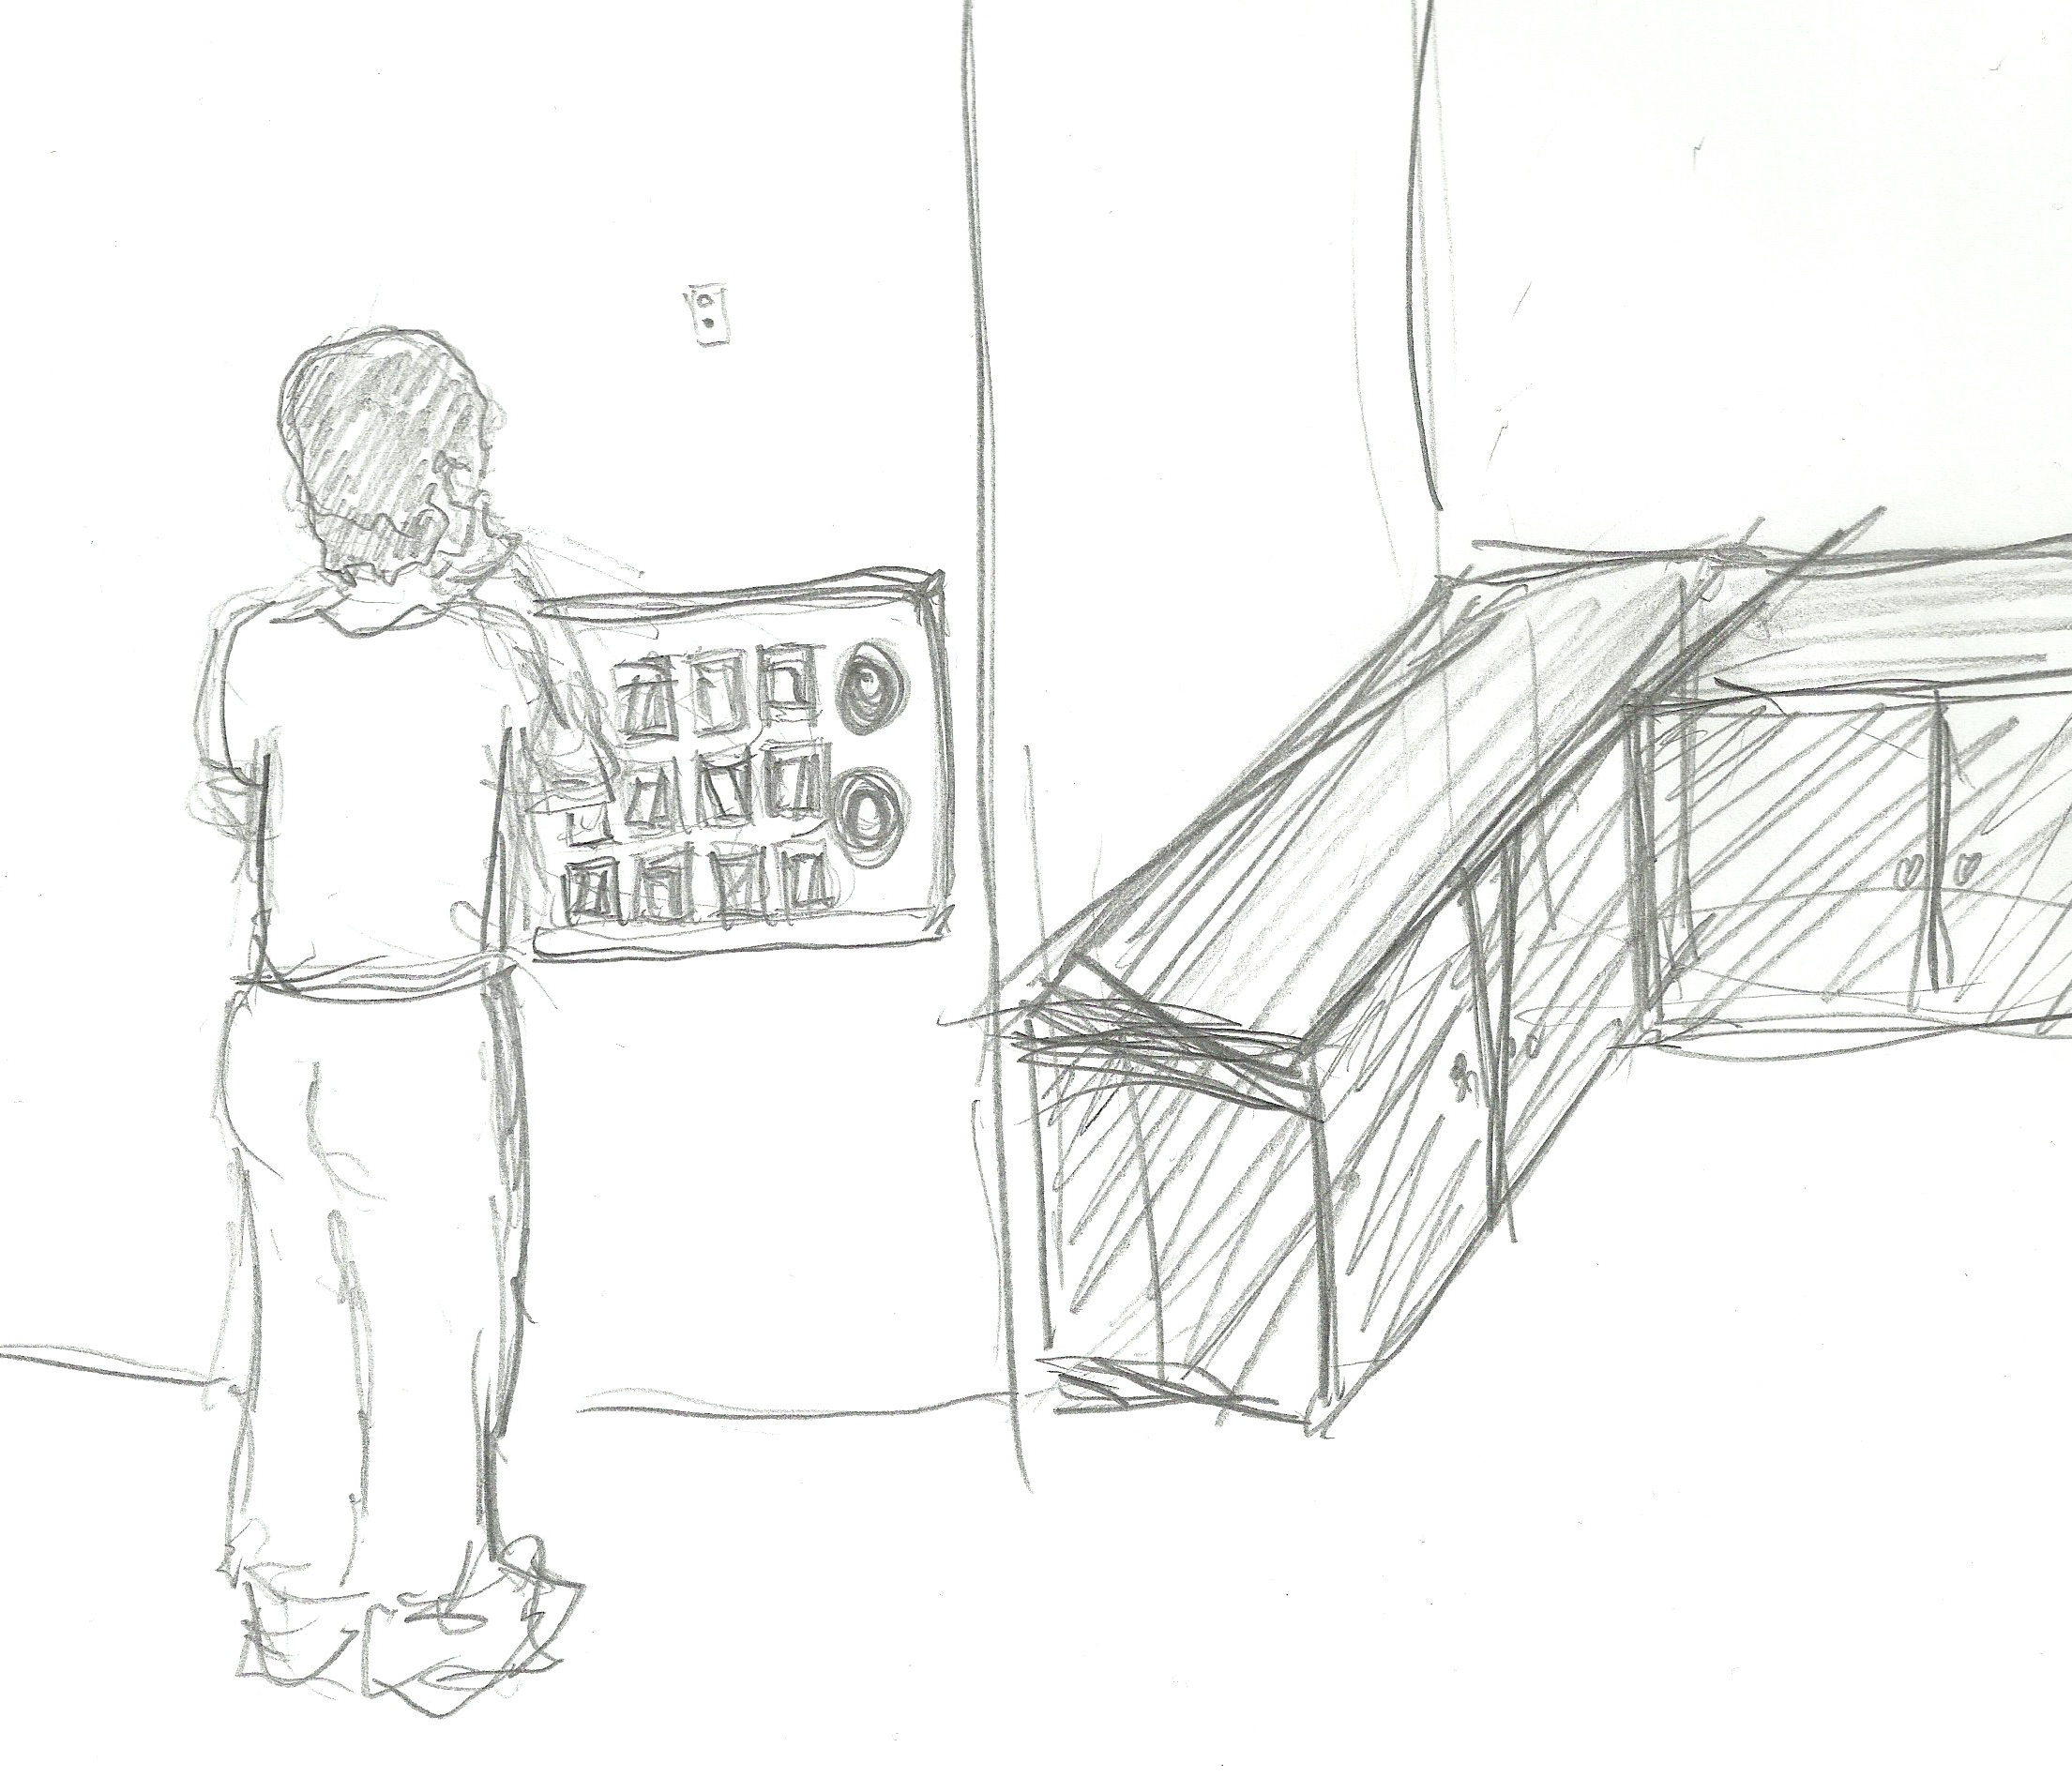
\includegraphics[scale=0.1]{fig/buttons}
\caption{En vegg med knapper skaper forvirring.}
\label{fig:panel}
\end{figure}

Dette kapittelet har følgende bidrag:
\begin{itemize}
\item Jeg argumenterer for at en gestesensor i form av enkle fotodioder er et tilstrekkelig medium for enkel brukerinteraksjon (\ref{ch:2.minide}).
\item Jeg viser at maskinlæring kan benyttes for å lære et system å forstå enkle gester og viser at dette er et alternativ til å eksplisitt programmere forståelse (\ref{ch:2.resultater}).
\item Jeg viser at det holder med et titalls treningseksempler fra hver gest for å oppnå gode resultater med lineære modeller og at det med 50 eksempler oppnås en suksessrate på 96\% (\ref{ch:2.resultater}).
\end{itemize}

\subsection{Interaksjon gjennom gester}
\label{ch:2.minide}
{\color{red}PING: Maskinlæring kan benyttes for å gi enkle sensorer en svært god forståelse av gester.}
Dette avsnittet presenterer hovedidéen for dette kapitellet. 
Dersom man ønsker å tilby styringsmuligheter på en eller flere vegger i et hus kan enkle gestesensorer benyttes i steden for et panel av knapper og dimmere. Selve sensoren er på størrelse med et knappenålshode og vi kan dermed forestille oss at designere kan komme opp med produktimplementasjoner som enten forsvinner inn i hjemmiljøet eller synes tydelig, men er praktisk og estetisk veldesignet. Sensoren merker at en hånd eller et annet objekt befinner seg foran den ved å sende ut et svakt infrarødt signal som reflekteres og detekteres dersom signalet er sterkt nok når det returnerer. Dette vil bare skje dersom objektet er opptil 20 cm unna sensoren. Dette betyr at gester kun forstås dersom de utføres rett foran sensoren. I motsetning til forståelse av gester gjennom bruk av kameraer er dette altså en langt mindre påtrengende måte å "lytte" etter innspill fra brukerne. Brukere kan være sikre på at de hverken overvåkes eller at personvernet deres på noen måte brytes. En slik gestesensor fungerer rett og slett kun som en multifunksjonell knapp.

\begin{wrapfigure}{r}{0.4\textwidth}
    \vspace{-20pt}
  \begin{center}
    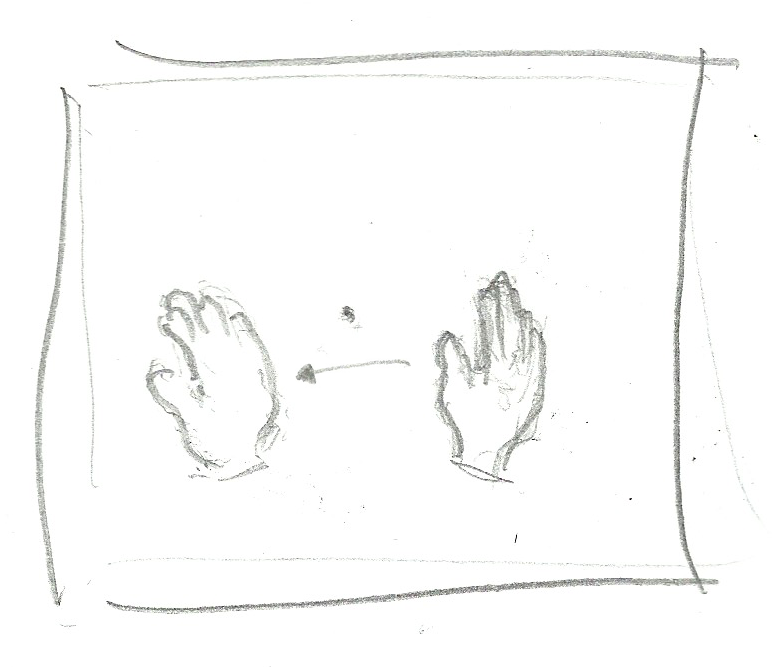
\includegraphics[width=0.35\textwidth]{fig/swipe-l-r}
  \end{center}
  \vspace{-20pt}
  \caption{Illustrasjon av en typisk gest.}
  \label{fig:gest}
  \vspace{-7pt}
\end{wrapfigure}

Figur \ref{fig:gest} viser en typisk gest der brukeren sveiper hånda foran sensoren som befinner seg på veggen. Vi kan forestille oss at denne sveipende bevegelsen foran denne sensoren betyr å skru av lyset i rommet sensoren befinner seg i. Men kanskje gesten betyr å skru på radioen, lukke gardinene eller starte kaffemaskinen. Det er ingen begrensning på hva en enkelt gest aktiverer i form av funksjonalitet.

Når en gest utføres må enten rådataene fra sensoren eller en forståelse av dataene sendes til en maskin som har ansvaret for å styre apparatene i hjemmet. Sensoren må være knyttet til en mikrokontroller eller tilsvarende som har ansvaret for å sende dataene videre. Dette kan enten være gjennom kabel eller trådløst. Det er mulig å programmere en mikrokontroller til å skille mellom sensordataene og forstå seks ulike gester {\color{red} ref}. Dette er i seg selv bra og betyr at en enkelt sensor kan fungere som en multifunksjonell knapp med minimum seks forskjellige kommandoer. Hvis man også utnytter at kombinasjonen av flere gester etter hverandre kan bety egne kommandoer er styringsmulighetene mange. Det finnes et alternativ til å programmere inn hva de ulike dataene skal tolkes som. Alternativet er å sende rådataene til en kraftigere maskin som kan benytte den spennende teknikken kjent som maskinlæring til å forstå enda flere ulike gester, med god sannsynlighet for suksess.

Maskinlæring handler om å la maskinen lære fra data. Dette kan enten være et forsøk på å finne ukjente sammenhenger i dataene den mates med eller det kan være å lære seg sammenhenger mellom dataeksempler og etiketter/klasser. Det er dette sistnevnte scenariet vi er interessert i. Vi kan mate maskinen med data fra en gest og samtidig gi informasjon om at dataene maskinen akkurat fikk betyr "sveip til høyre". Dermed kan maskinen danne en kobling mellom dataene som kom inn da vi sveipet til høyre og etiketten "sveip til høyre". Med tilstrekkelig treningseksempler fra de ulike gestene skal maskinen kunne lære seg forskjellene mellom de ulike gestene. Dermed vil den være i stand til å gjette riktig på hvilken gest vi utfører ved en senere anledning. Prototypen jeg har utviklet er trent med 50 ulike dataeksempler på hver av de 10 ulike gestene.

\begin{figure}[h]
\begin{subfigure}{0.23\textwidth}
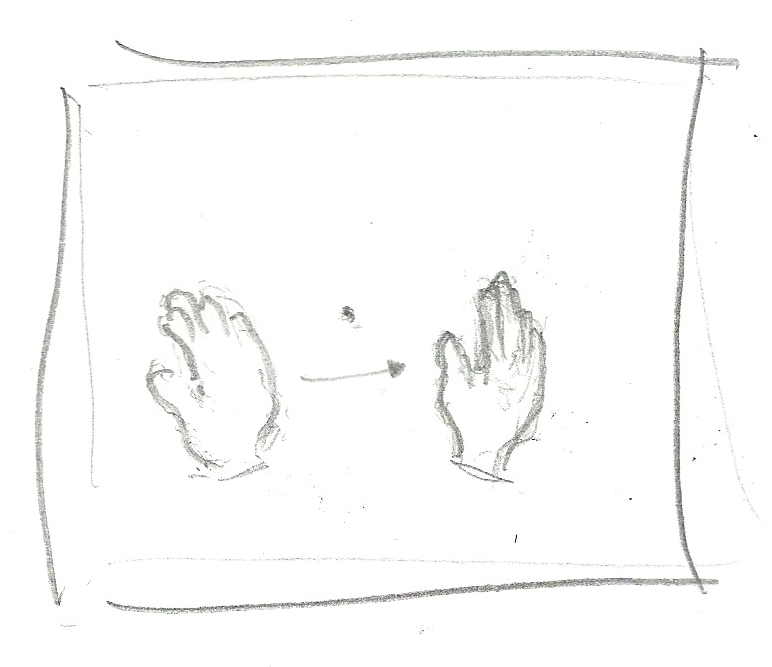
\includegraphics[width=3cm, height=3cm]{fig/swipe-r-l}
\caption{Sveip til høyre.}
\label{fig:sveip-}
\end{subfigure} 
\begin{subfigure}{0.23\textwidth}
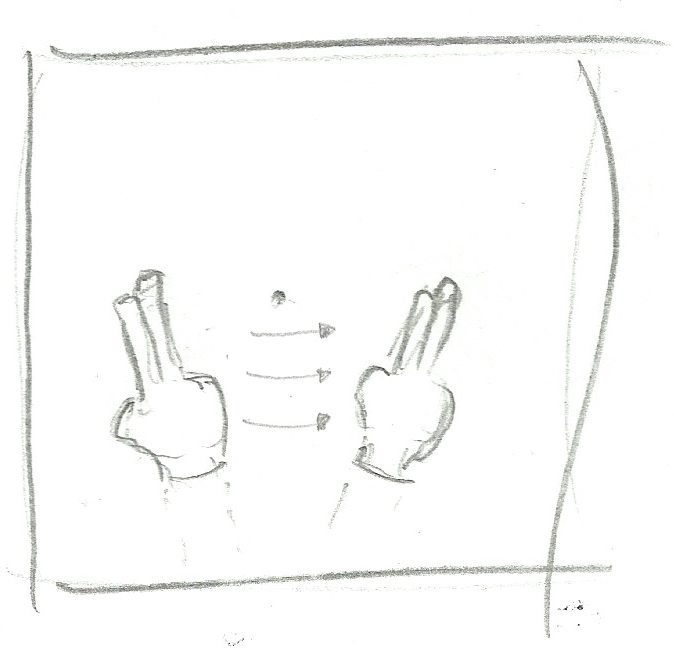
\includegraphics[width=3cm, height=3cm]{fig/flick-l-r} 
\caption{Flikk til høyre.}
\label{fig:flikk-h}
\end{subfigure}
\begin{subfigure}{0.23\textwidth}
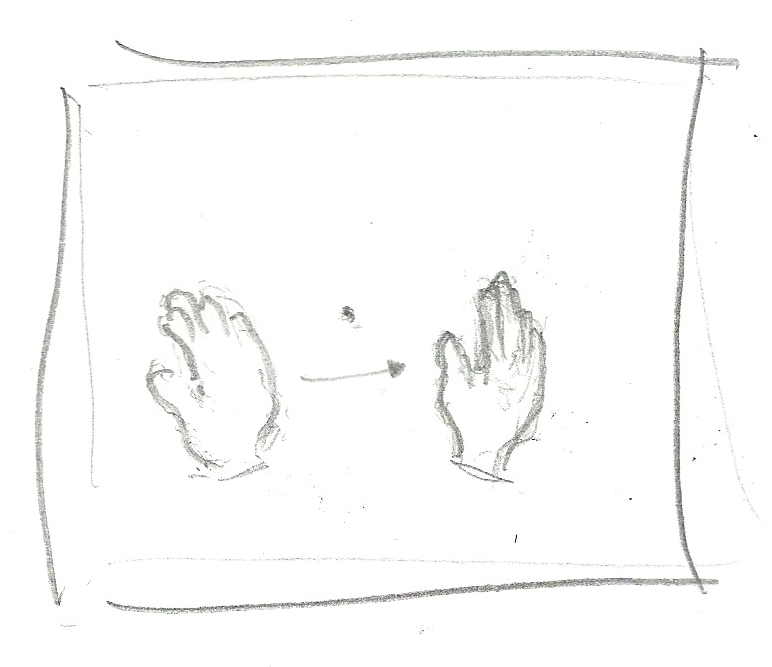
\includegraphics[width=3cm, height=3cm]{fig/swipe-r-l}
\caption{Sveip til venstre.}
\label{fig:sveip-v}
\end{subfigure} 
\begin{subfigure}{0.23\textwidth}
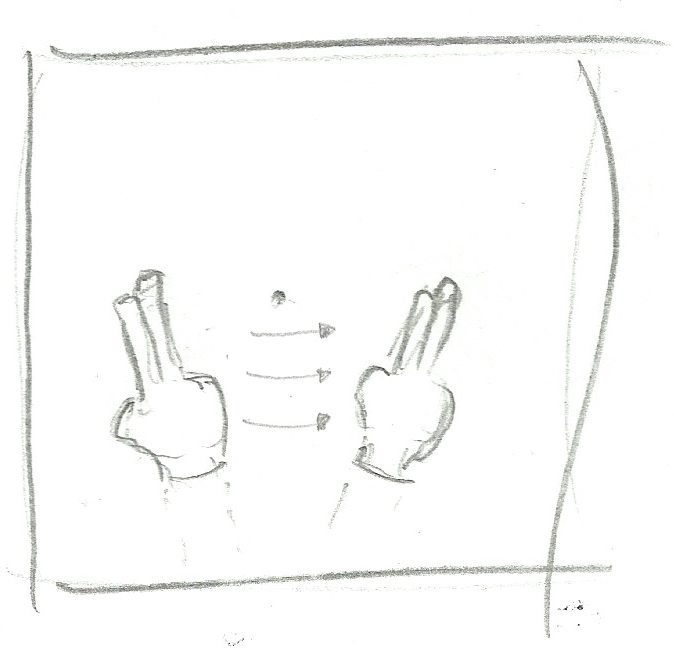
\includegraphics[width=3cm, height=3cm]{fig/flick-l-r}
\caption{Flikk til venstre.}
\label{fig:flikk-v}
\end{subfigure}
\begin{subfigure}{0.23\textwidth}
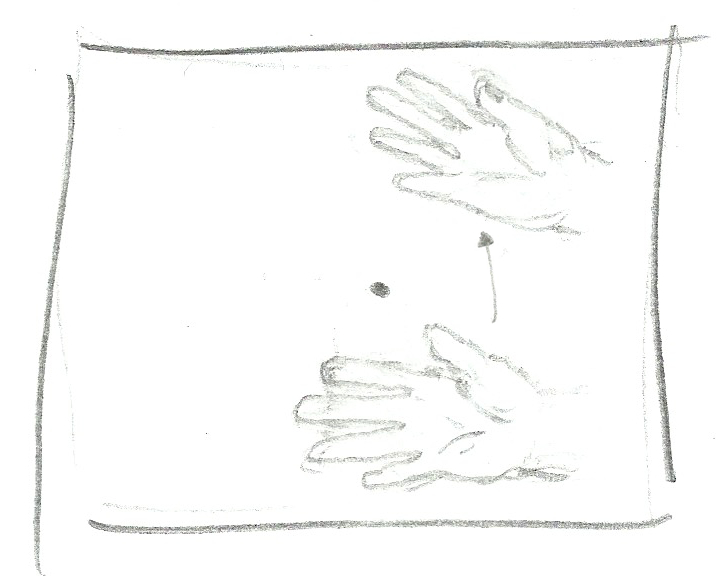
\includegraphics[width=3cm, height=3cm]{fig/swipe-d-u}
\caption{Sveip opp.}
\label{fig:sveip-opp}
\end{subfigure}
\begin{subfigure}{0.23\textwidth}
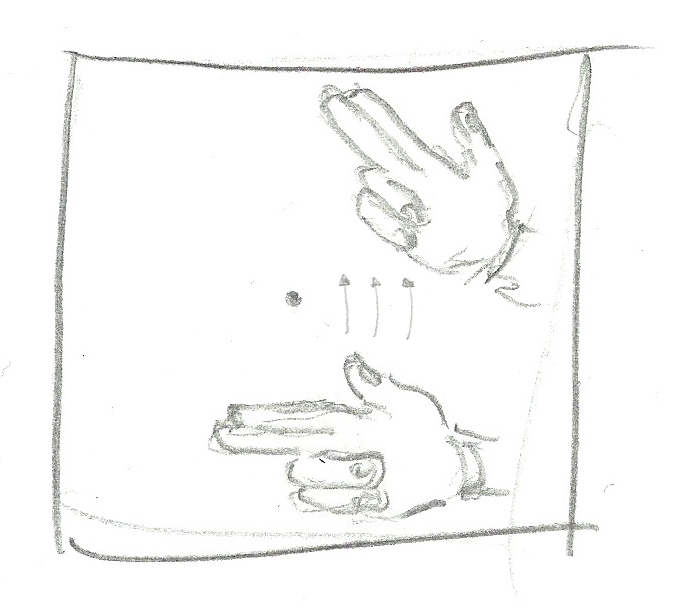
\includegraphics[width=3cm, height=3cm]{fig/flick-d-u}
\caption{Flikk opp.}
\label{fig:flikk-opp}
\end{subfigure}
\begin{subfigure}{0.23\textwidth}
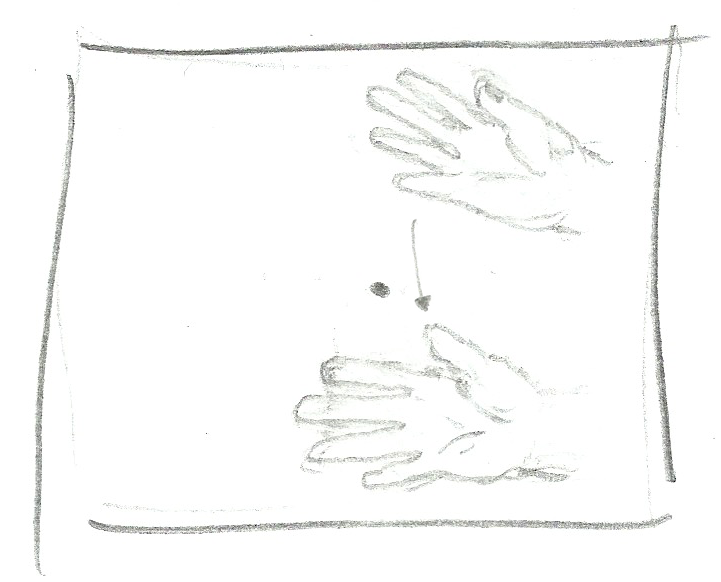
\includegraphics[width=3cm, height=3cm]{fig/swipe-u-d}
\caption{Sveip ned.}
\label{fig:sveip-ned}
\end{subfigure}
\begin{subfigure}{0.23\textwidth}
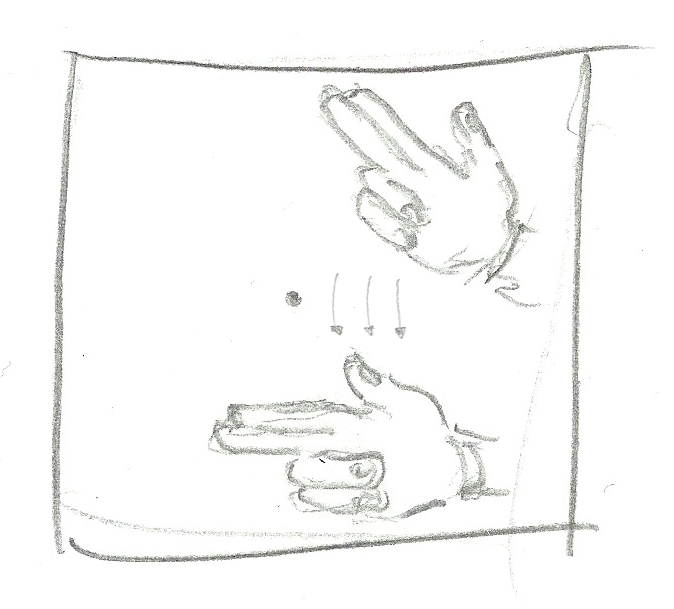
\includegraphics[width=3cm, height=3cm]{fig/flick-u-d}
\caption{Flikk ned.}
\label{fig:flikk-ned}
\end{subfigure}
\begin{subfigure}{0.25\textwidth}
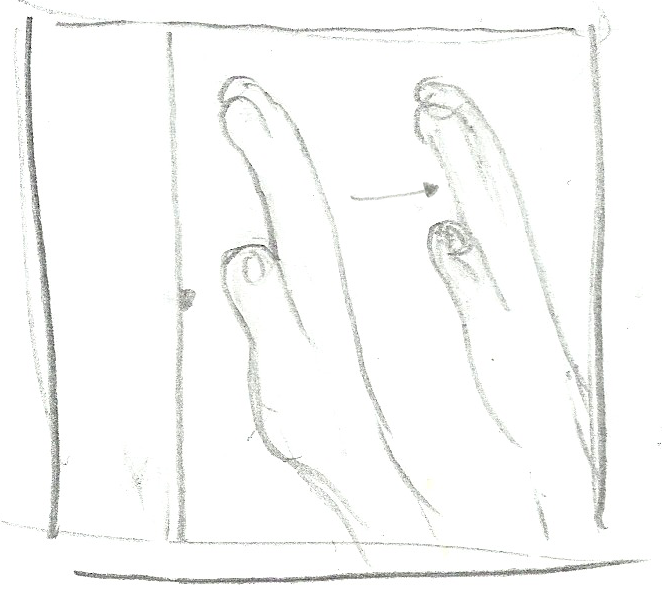
\includegraphics[width=3cm, height=3cm]{fig/near-far}
\caption{Nær - fjern.}
\label{fig:n-f}
\end{subfigure}
\begin{subfigure}{0.23\textwidth}
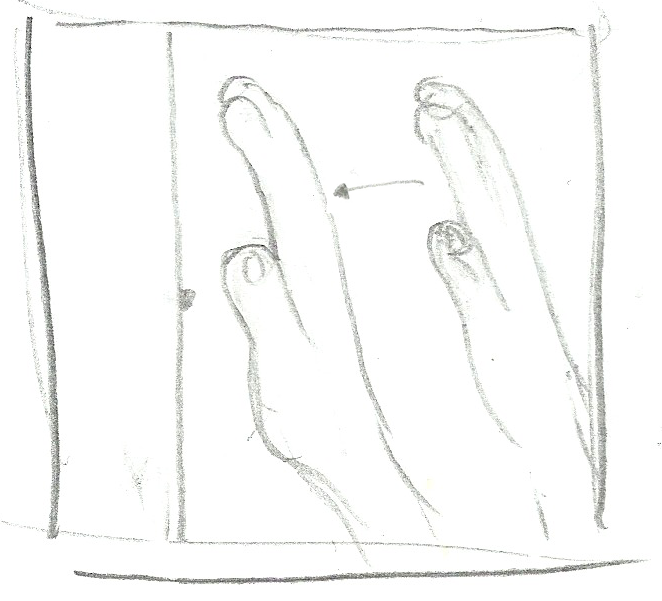
\includegraphics[width=3cm, height=3cm]{fig/far-near}
\caption{Fjern - nær.}
\label{fig:f-n}
\end{subfigure}
\caption{Illustrasjoner av de ulike gestene.}
\label{fig:gester}
\end{figure}

\subsection{Detaljer}
\subsubsection{Hardware}
Sensoren som benyttes i denne prototypen er APDS-9960 fra Avago Technologies. Sensoren tilbyr måling av lys og farge, oppdagelse av nærhet og gestegjenkjennelse\footnote{Kapittel 4 utforsker bruksområder for funksjonaliteten rundt lys, farge og nærhet.}. Innpakningen er svært liten på kun 3.94 * 2.36 * 1.35 mm. Selve gestesensoren består av fire fotodioder som merker et reflektert infrarødt signal utsendt fra en LED. Fotodiodene er vinklet litt forskjellig slik at de plukker opp refleksjoner på litt forskjellige steder. Den benytter resultater fra nærhetsdetektoren for å automatisk aktiveres når et objekt er innen rekkevidde. I tilegg brukes måling av lys for å tilpasse de infrarøde målingene til lysnivået i omgivelsene. Dataene dannes som 32-bit datasett og kommuniseres over I2C-protokollen til en mikrokontroller. Gestesensoren kan selv håndtere forståelse av gester som passerer opp, ned, mot venstre eller mot høyre over sensoren, men denne funksjonaliteten tar vi ikke i bruk her {\color{red} ref apds9960-dokumentasjonen.}.

Prototypen er utviklet med Sparkfun's innpakning av APDS9960-sensoren\footnote{https://www.sparkfun.com/products/12787}. Denne brettet gjør APDS9960-sensoren tilgjengelig for enkel prototyping ved å bryte ut ulike pinner. {\color{red} bilde av sparkfun-brikken som peker ut hvilken del som er apds9960.} I tillegg har de gjort tilgjengelig programvare til Arduino-plattformen\footnote{http://www.arduino.cc/} så utviklere kommer raskt i gang. De ulike programmene som kan lastes opp til en Arduino gir tilgang til de forskjellige funksjonalitetene hos APDS-9960-brikken.

\subsubsection{Dataprosessering}
Seriell data sendes fra mikrokontrolleren til datamaskinen som lytter på riktig port. Sensoren sender data så lenge ir-signalet reflekteres. Dette betyr at en gest som tar lengre tid skaper mer data. Et rolig sveip over sensoren med hele hånda kan skape 100-200 datapunkter. Et raskt flikk med to fingre skaper 16-32 datapunkter. En gest som involverer å holde hånda foran sensoren i et sekund eller mer skaper flere hundre datapunkter. For å benytte de planlagte klassifiseringsteknikkene må hvert av treningseksemplene må ha like mange egenskaper.

Det finnes ulike metoder for å løse dette problemet. En av de er å bestemme et øvre antall maksimale egenskaper som skal tas med. Inputeksempler som ikke har tilstrekkelig med egenskaper blir paddet med 0-verdier. Å sette en maksgrense på egenskaper kan føre til at man mister viktig data fra gester som tar lengre tid å utføre. For et inputeksempel fra en rask gest vil mange egenskaper være 0. Dette kan påvirke effektiviteten til læringsalgoritmen. Et annet alternativ er å velge et fast antall egenskaper vært inputeksempel skal ha og så knytte inputeksempelet til denne egenskapervektoren. Dersom inputdataene har få datapunkter blir egenskapsvektoren sparsom, med dataverdiene spredt jevnt utover og med 0-verdier i mellom. Dersom inputdataene består av mange datapunkter vil hver egenskap i egenskapsvektoren være et gjennomsnitt av en valgt mengde datapunkter.

Jeg valgte å benytte denne sistnevnte teknikken og lagde vektorer med 128 egenskaper. Dette tallet ble valgt basert på antall datapunkter som genereres ved ulike aktuelle gester. 128 egenskaper er nok til å gi tilstrekkelig detaljer selv ved gester som tar noe lengre tid og samtidig ikke så mange at raske gester skaper i overkant sparsomme vektorer. Egenskapsvektoren normaliseres ved å knytte de mulige sensorverdiene [0,255] til [0,1.0]. Å illustrere dannelsen av vektorere med 128 egenskaper blir tungvint så i figur \ref{fig:data} har jeg illustrert prosessen med mindre data. I \ref{fig:few} består inputvektoren av to datapunkter. Vi ønsker en egenskapsvektor med størrelse fire. Dette oppnås ved å spre inputdataene jevnt i egenskapsvektoren og normalisere verdiene. \ref{fig:many} viser det motsatte tilfellet, der inputvektoren er for stor. For å representere dataene i en mindre egenskapsvektor blir det tatt gjennomsnittsverdier som deretter normaliseres. 

\begin{figure}[h]
\centering
\begin{subfigure}{0.23\textwidth}
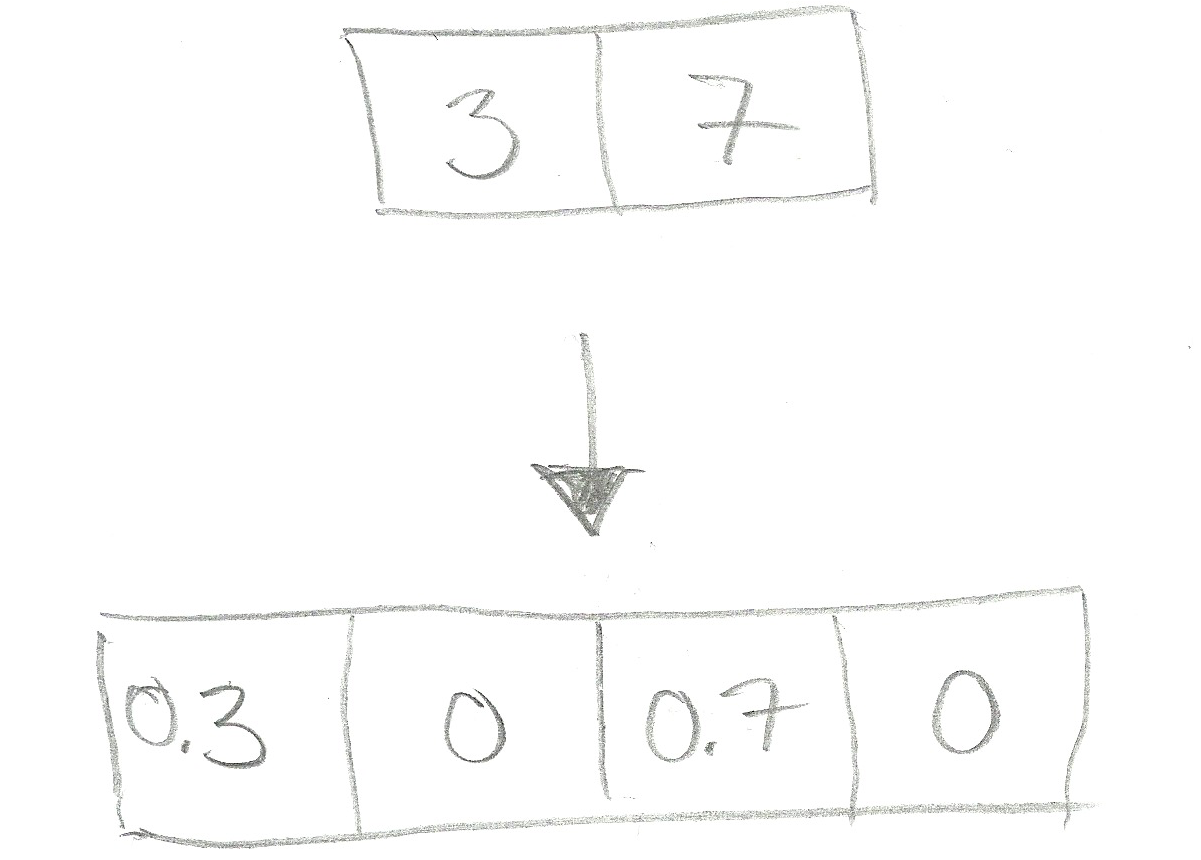
\includegraphics[width=3cm, height=3cm]{fig/few-to-many}
\caption{}
\label{fig:few}
\end{subfigure}
\begin{subfigure}{0.23\textwidth}
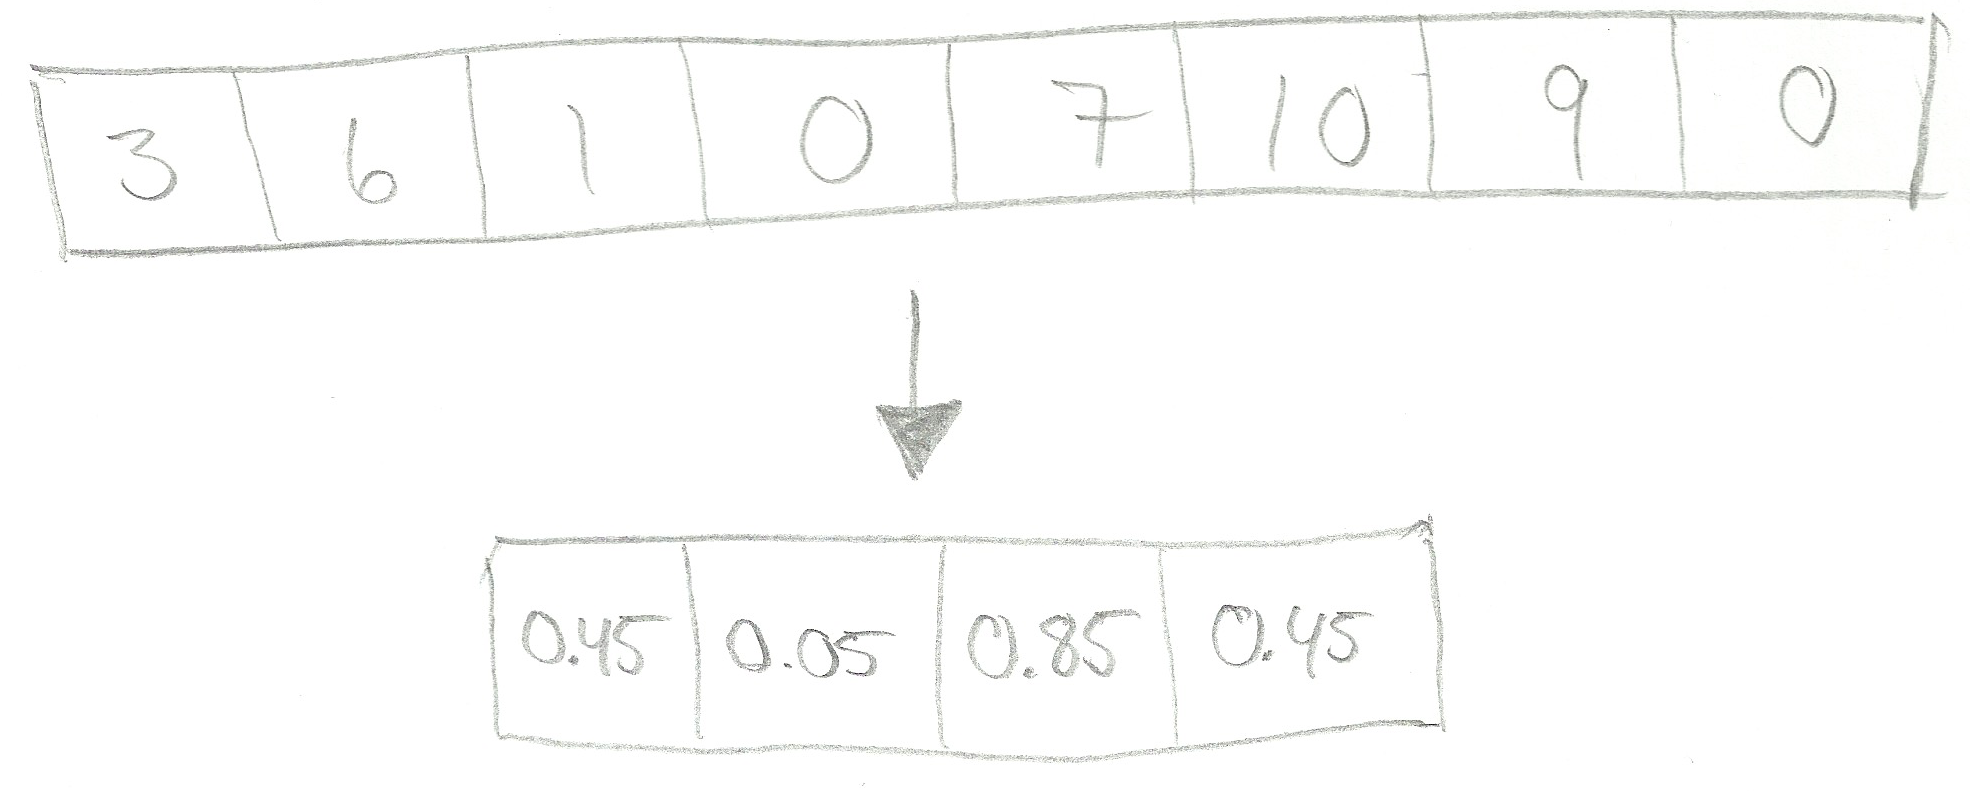
\includegraphics[width=3cm, height=3cm]{fig/many-to-few}
\caption{}
\label{fig:many}
\end{subfigure}
\caption{Illustrasjon av dannelsen av en egenskapsvektorer.}
\label{fig:data}
\end{figure}

{\color{red} ref process-data.py/trim-data}

\subsubsection{Maskinlæring: Klassifisering}
La oss begynne med en definisjon på maskinlæring fra Arthur Samuel (1959): "Maskinlæring gir datamaskiner evnen til å lære uten å bli eksplisitt programmert."

Denne definisjonen er over 50 år gammel, men den fanger hva vi er ute etter. Vi er interessert i å få datamaskinene til å lære å gjøre nyttige ting uten å behøve å fortelle dem eksplisitt hvordan hver enkelt oppgave skal utføres. Dette er nødvendig da det med mye og kompleks data raskt blir umulig for en programmerer å beskrive alle deloppgavene som må utføres.

Alle maskinlæringsproblemer kan konseptualiseres som å finne en funksjon som knytter input til output. Målet kan være å tilnærme en enkel matematisk funksjon, det kan være å spå aksjekursen basert på historisk data eller det kan være å gi sannsynligheten for et en epost er spam, basert på innholdet. Man tar erfaring, i form av empirisk data, og kjører det gjennom en algoritme som forsøker å finne en funksjon som dekker denne kunnskapen best mulig.

I dette prosjektet skal dataene en gest danner knyttes til navnet på en gest. Dette er en form for maskinlæring kalt overvåket læring. Målet er å klassifisere nye data korrekt, basert på treningsgrunnlaget fra tidligere data. Læringen sies å være overvåket fordi vi bidrar med informasjon om hvilke klasser som hører til hvilke data i treningseksemplene. Framgangsmåten er å mate maskinen med mange eksempler på denne koblingen mellom data og gest og håpe at maskinen finner en matematisk funksjon som tilnærmer denne sammenhengen godt.

Dataene vi jobber med i dette prosjektet har 128 egenskaper og 50 treningseksempler av hver klasse. Dette er relativt mange egenskaper og få treningseksempler. Basert på disse karakteristikkene er det sannsynlig at enkle, lineære modeller vil gi de beste resultatene {\color{red} refeefer! Scikitlearn?}. Mer avanserte klassifiseringsteknikker, som for eksempel nevrale nettverk, kan i teorien tilnærme enhver funksjon, men de trenger langt flere treningseksempler for å finne de sanne sammenhengene mellom datapunktene.

Vi mater et treningssett av datapunkter til en valgt læringsalgoritme. Algoritmen danner seg en hypotese om hva slags modell som best beskriver dataene. Denne hypotesen kan så benyttes til å gjøre gjetninger på nye datapunkter. Hypotesen avhenger av egenskapene i datapunktene. I en lineær modell er hypotesen en funksjon av egenskapene $x$ i treningsdataene, der hver egenskap blir vektet av $\theta$-verdier:

\begin{equation}
h_\theta(x) = \theta_0x_0 + \theta_1x_1 + \theta_2x_2 + ... + \theta_nx_n
\label{eq:hypotese-lin}
\end{equation}

I dette prosjektet har hvert datapunkt $n = 128$ egenskaper. La oss modellere $x$ til å være en vektor med disse egenskapene: 
\[
x =
\begin{bmatrix}
x_0 \\
x_1 \\
x_2 \\
.. \\
x_{128}
\end{bmatrix}
\in R^{128},
\]
Vi lar $\theta$ være en tilsvarende vektor: 
\[
\theta =
\begin{bmatrix}
\theta_0 \\
\theta_1 \\
\theta_2 \\
.. \\
\theta_{128}
\end{bmatrix}
\in R^{128}
\]

Dersom vi nå tar den transponerte av $\theta$ og lar \(x_0 = 1\), kan vi i stedet for (\ref{eq:hypotese-lin}) skrive hypotesen elegant og kompakt som indreproduktet av vektorene:
\begin{equation}
h_\theta(x) = \theta^{T}x
\label{eq:hypotese-kompakt}
\end{equation}

En vellykket hypotese vekter $\theta$-verdiene slik at algoritmen gir de beste mulige resultatene. Denne vekttingen tilsvarer det å finne hvilke egenskaper i dataene som er de viktigste for å angi hvilken klasse dataeksempelet tilhører. Så hvordan velger man disse $\theta$-verdiene? Vi ønsker $\theta$-verdier slik at hypotesen \(h_\theta(x)\) er nære klassen $y$, for treningseksemplene \((x,y)\). Treningseksemplene  \((x,y)\) representerer eksempelkoblinger mellom data og klasse. Dersom vi antar at hypotesen er en lineær funksjon og at dataene kun har to egenskaper, kan vi plotte hypotesen som en linje gjennom datapunktene. For hvert nye treningseksempel algoritmen prosesserer vil $\theta$-verdiene justeres og linjen vil tilpasses til å følge datapunktene som angir en av de to klassene bedre. Etter at funksjonen er trent på en rekke treningseksempler vil linjen forhåpentligvis danne et klart skille mellom datapunktene som utgir de to klassene (se figur \ref{figure:separator}).

\begin{figure}[h!]
\centering
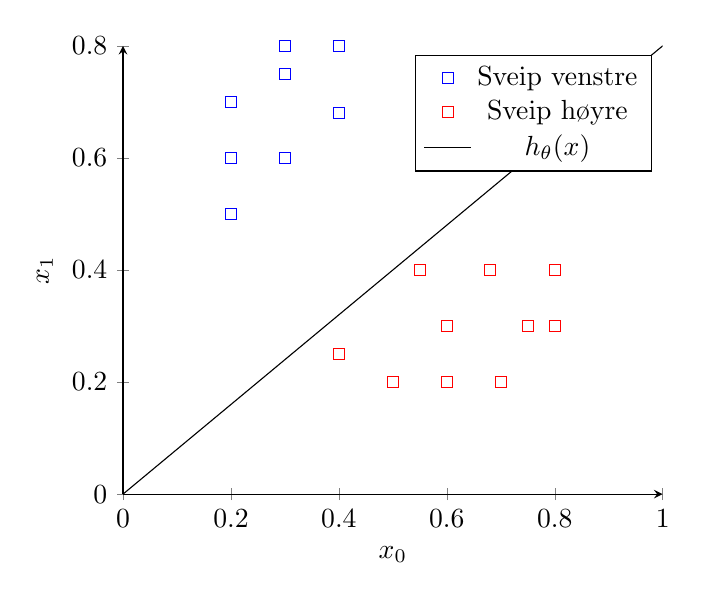
\begin{tikzpicture}
\begin{axis}[
    axis lines = left,
    xlabel = $x_0$,
    ylabel = {$x_1$},
]
\addplot[
    only marks,
    color=blue,
    mark=square,
    ]
    coordinates {
    (0.2,0.7)(0.2,0.5)(0.2,0.6)(0.3,0.8)(0.3,0.6)(0.3,0.75)(0.4,0.8)(0.4,0.68)
    };
\addlegendentry{Sveip venstre}
\addplot[
    only marks,
    color=red,
    mark=square,
    ]
    coordinates {
    (0.55,0.4)(0.4,0.25)(0.7,0.2)(0.5,0.2)(0.6,0.2)(0.8,0.3)(0.6,0.3)(0.75,0.3)(0.8,0.4)(0.68,0.4)
    };
\addlegendentry{Sveip høyre}
\addplot [
    domain=0:1, 
    samples=100, 
    color=black,
]
{0.8*x};
\addlegendentry{\(h_\theta(x)\)}
\end{axis}
\end{tikzpicture}
\caption{Plot av en lineær hypotese som deler datapunktene i to tilhørende klasser.}
\label{figure:separator}
\end{figure}

Separatoren i figur \ref{figure:separator} er en linje i to dimensjoner. En separator i tre dimensjoner vil danne et plan. Det blir deretter vanskelig for oss å forestille oss en separator som opererer i mer enn tre dimensjoner. Heldigvis kommer matematikken til vår hjelp da den ikke bryr seg om våre visuelle begrensninger og fungerer like godt i 128 dimensjoner som i tre. Vi har konkludert med at en lineær modell bør få sjansen til å skille dataeksemplene våre, men hvilken algoritme bør vi benytte? To lignende, mye brukte og robuste teknikker er logistisk regresjon og støttevektormaskiner.

\subsubsection*{Logistisk regresjon}
I logistisk regresjon modelleres sannsynlighetene som beskriver ulike utfall av en logistisk sigmoid-funksjon som gir verdier i området \([0,1]\). Figur \ref{figure:sigmoid} viser den generelle sigmoid-funksjonen. Vi ser at ved større positive x-verdier gir funksjonen et resultat nære 1, mens for større negative verdier gir funksjonen et resultat nære 0.

\begin{equation}
g(x) = \frac{1}{1 + e^{-x}}
\label{eq:sigmoid}
\end{equation}

\begin{figure}[h!]
\centering
\begin{tikzpicture}
\begin{axis}[
    axis lines = center,
    xlabel = $x$,
    ylabel = {$y$},
]
\addplot [
    domain=-5:5, 
    samples=100, 
    color=red,
]
{1 / (1 + e^(-x))};
%\addlegendentry{\(g(x) = \frac{1}{1 + e^{-x}}\)}
\end{axis}
\end{tikzpicture}
\caption{Plot av en ordinær sigmoidfunksjon.}
\label{figure:sigmoid}
\end{figure}

La oss si vi har to mulige klasser, \(y \in \{0,1\}\). Hvis \( h_\theta(x) \geq  0.5\), gjetter vi at klassen \(y = 1\). Hvis \( h_\theta(x) < 0.5\), gjetter vi \(y = 0\).

Når vi nå kombinerer (\ref{eq:hypotese-kompakt}) og (\ref{eq:sigmoid}) får vi den logistiske hypotesen \ref{eq:logistic}.

\begin{equation}
h_\theta(x) = \frac{1}{1 + e^{-\theta^{T}x}}
\label{eq:logistic}
\end{equation}

Igjen representerer $\theta$ vektingen av egenskapene $x$ i treningsdataene. For å tilpasse $\theta$-verdiene er strategien å minimere en kostnadsfunksjon definert av forskjellen mellom hva hypotesen gjetter og hva som var det riktige svaret. Kostnadsfunksjonen er en variant av minste kvadrats metode {\color{red}ref Kreyzig(?)} \ref{eq:minimize}. 

\begin{equation}
J(\theta) = 
    \frac{1}{2m} \sum_{i=1}^{m} (h_\theta(x^{(i)})-y^{(i)})^2
\label{eq:minimize}
\end{equation}

For å minimere denne kostnadsfunksjonen brukes en oppdateringsregel. Regelen oppdaterer egenskapsvektoren $\theta$ ved å trekke fra resultatet fra den partiellderiverte av kostnadsfunksjonen, dempet av en faktor $\alpha$:

\begin{equation}
\theta_j \leftarrow \theta_j - \alpha \frac{\delta}{\delta\theta_j}J(\theta)
\label{eq:gradient}
\end{equation}

Ettersom den deriverte i et gitt punkt er brattheten til kurven i det punktet vil denne oppdateringen tilsvare å stadig ta mindre steg i den retningen som fører mot en lavere verdi på kurven. På en to-dimensjonell graf vil det si å følge plottet nedover mot et bunnpunkt, men algoritmen fungerer på samme vis i høyere dimensjoner. Denne oppdateringsregelen kalles gjerne "gradient descent" og brukes i flere maskinlærings-sammenhenger for å finne minimumsverdier.

For å lære å skille mellom de 10 ulike klassene benyttes strategien "en-mot-resten". For hver klasse trenes det en egen hypotese som best mulig skiller mellom denne klassen og alle de andre. I vårt tilfelle betyr dette at vi trener 10 hypoteser. Når ny data kommer inn til det trente systemet velges den hypotesen blant de 10 som gir den høyeste sannsynligheten for en viss klassifisering og dermed er mest sikker på å ha funnet det riktige svaret.

\subsubsection*{Støttevektormaskiner (SVM)}
Støttevektormaskiner er en gruppe overvåkede maskinlæringsalgoritmer som kan brukes til å løse klassifiseringsproblemer. De er kjent for å være effektive i problemområder med mange dimensjoner og kan oppnå gode resultater selv når antallet dimensjoner er høyere enn treningseksemplene. De bruker mindre plass i minnet enn andre tilnærminger og kan tilpasses til å løse en rekke forskjellige problemer. En ulempe med SVM'er er at de ikke tilbyr direkte estimater på hvor sikker klassifiseringen er og at de i utgangspunktet bare kan skille mellom to klasser.

En støttevektormaskin danner et hyperplan eller et sett av hyperplan i et høydimensjonelt rom. Disse hyperplanene brukes for å danne skiller mellom data og kan dermed brukes til klassifisering. En optimal deling oppnås av hyperplanet som har den største avstanden til det nærmeste datapunktet til en klasse. Generelt vil den største marginen mellom klassene senke klassifikatorens feilaktighet.

Math.

Plot.

For å håndtere klassifisering av flere klasser finnes det ulike strategier.

En-mot-en (Knerr et al., 1990). Dersom n er antallet klasser trenes n * n-1 / 2 klassifiserere. Hver av disse trenes med data fra to klasser. 10*9 / 2 gir 45.

En-mot-resten, trener n klassemodeller, gir 10.

\subsubsection{Eksperimentsutførelse}
For å trene klassifikatorer kreves data. Arduinoen kobles til maskinen med en usb-kabel. Arduino-biblioteket har blitt forandret minimalt til å ikke selv forstå sensordataene, men i stedet dytte dem videre til datamaskinen. Et Python-script åpner tilkoblingen til å lytte på en seriell port. Porten åpnes i noen sekunder og ber om at en gest utføres {\color{red} ref process-data.py}. Jeg gjennomførte 50 utførelser av hver av de 10 gestene og lagret dataene for hver gest i hver sin csv-fil. Med dataene for hver gest lagret i forskjellige filer kan disse kombineres slik man ønsker for å trene systemet til å skille mellom 2,3, eller opp til 10 gester. 

Splitte dataene, trene med 75\% og teste med 25\%. Dette er en viktig øvelse for å ikke spesialisere modellen til dataene. Dersom man trener på hele datasettet og tester på det samme settet er det en sjanse for at man har tilpasset modellen for mye til datasettet og ikke funnet den underliggende, generelle modellen. Dette kalles "overfitting". {\color{red} ref learning.py}

\subsubsection{Resultater}
\label{ch:2.resultater}
\begin{table}[h!]
\centering
\begin{tabular}{|| c c c ||}
\hline
\% Korrekt klassifisering & Algoritme & Antall treningseksempler\\ [0.5ex] 
 \hline\hline
 96,0 & SVM m/libsvm & 500 \\ 
 \hline
 95,8 & SVM m/liblinear & 500 \\
 \hline
 94,048 & Logistisk regresjon & 500 \\ [1ex]
 \hline
\end{tabular}
\caption{Gjennomsnittsresultater for klassifisering der modellene er trent og testet 100 ganger med tilfeldige utgangspunkt.}
\label{table:results}
\end{table}

%http://www.csie.ntu.edu.tw/~cjlin/papers/libsvm.pdf
%http://www.csie.ntu.edu.tw/~cjlin/papers/liblinear.pdf
%http://www.csie.ntu.edu.tw/~cjlin/papers/maxent_dual.pdf
%http://www.farnell.com/datasheets/1801560.pdf

96\% er et svært godt resultat og viser hvor godt enkle lineære modeller kan skille mellom denne typen data. Det er interessant å spørre seg om dette resultatet kunne blitt enda høyere. Jeg valgte derfor å gjøre det samme eksperimentet med en femtedel og halvparten av dataene. Dette for å se sammenhengen mellom forbedring i suksessrate og antall treningseksempler. Ettersom scikit-learn-biblioteket tilbyr en rekke algoritmer har jeg forsøkt andre tilnærminger enn lineære modeller og inkludert dem også. Figur\ref{figure:resultsgraf} viser resultatene for 100, 250 og 500 treningseksempler.

\begin{figure}[h!]
\centering
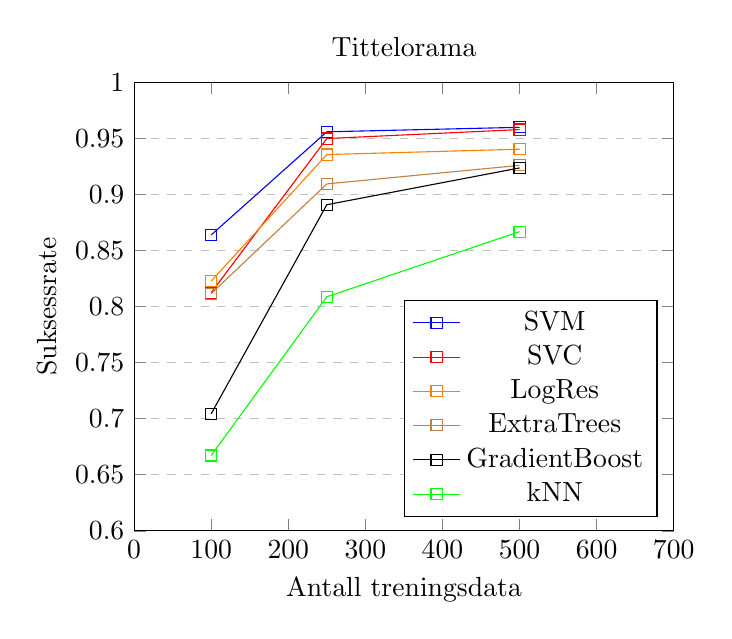
\begin{tikzpicture}
\begin{axis}[
    title={Tittelorama},
    xlabel={Antall treningsdata},
    ylabel={Suksessrate},
    xmin=0, xmax=700,
    ymin=0.6, ymax=1.0,
    xtick={0,100,200,300,400,500,600,700},
    ytick={0.6,0.65,0.7,0.75,0.8,0.85,0.9,0.95,1.0},
    legend pos=south east,
    ymajorgrids=true,
    grid style=dashed,
]
\addplot[
    color=blue,
    mark=square,
    ]
    coordinates {
    (100,0.864)(250,0.956)(500,0.96)
    };
\addplot[
    color=red,
    mark=square,
    ]
    coordinates {
    (100,0.8124)(250,0.95)(500,0.958)
    };
\addplot[
    color=orange,
    mark=square,
    ]
    coordinates {
    (100,0.8228)(250,0.9357)(500,0.94048)
    };
\addplot[
    color=brown,
    mark=square,
    ]
    coordinates {
    (100,0.8116)(250,0.9095)(500,0.92608)
    };
\addplot[
    color=black,
    mark=square,
    ]
    coordinates {
    (100,0.7044)(250,0.89095)(500,0.92376)
    };
\addplot[
    color=green,
    mark=square,
    ]
    coordinates {
    (100,0.6672)(250,0.8088)(500,0.86688)
    };
    
    \legend{SVM,SVC,LogRes,ExtraTrees,GradientBoost,kNN}
\end{axis}
\end{tikzpicture}
\label{figure:resultsgraf}
\caption{Resultatsutvikling for et utvalg algoritmer.}
\end{figure}

\subsection{Relatert arbeid}
{\color{red} 1-2 sider, utforskning av hva andre har gjort... Maskinlæring på sensordata fra gester (video)}

\subsection{Konklusjoner og videre arbeid}
Blablabla suksess!

I figur \ref{figure:resultsgraf} kan vi se at SVM'ene er i nærheten av 95\% allerede etter 250 treningseksempler og at de kun øker minimalt med 250 ekstra tilfeller. Dette tyder på at det trengs et svært antall ekstra treningseksempler for at algoritmene skal krype betydelig nærmere 100\%. De avanserte ExtraTrees og GradientBoost, benytter seg av kombinasjonsstrategier og flere teknikker. Det kan se ut som om spesielt GradientBoost kan fortsette å øke suksessraten betydelig med mer trening, men det er tvilsomt om den passerer SVM. Til sist nevnes k-næreste nabo, som begynner svakest av disse, men fremdeles har en sterk vekst mellom 250 og 500 tilfeller. Det hadde vært interessant å se utviklingen videre for denne enkle algoritmen.

Hva kan gjøres videre: online læring, flere gester (er det nyttig?), større egenskapvektor (enn 128) fordeler ulemper.



